\documentclass[11pt,letterpaper,fleqn]{article}
\usepackage{graphicx}
\usepackage{tabulary}
\usepackage{lineno}
\usepackage{hyperref}
\usepackage{subfigure}
\usepackage{cite}
\usepackage{xcolor,colortbl}
\usepackage{wrapfig}
\usepackage{enumitem} %%% uncommenting this line and associated
%% options only saves about 1/4 page
% enumitem options
%\setlist{nosep}
%\setitemize{wide}
%\setlist[itemize]{leftmargin=*}
%\setlist[enumerate]{leftmargin=*}

\selectcolormodel{rgb}
\definecolor{LHCb dark}{rgb}{0.0000,0.3412,0.6549}%From LHCb logo
\definecolor{UC red}{rgb}{0.8196,0.1176,0.2314} % from logo
\definecolor{brickred}{rgb}{0.8, 0.25, 0.33}
\definecolor{Gray}{gray}{0.85}
\definecolor{applegreen}{rgb}{0.55, 0.71, 0.0}
\definecolor{asparagus}{rgb}{0.53, 0.66, 0.42}
\definecolor{cadmiumgreen}{rgb}{0.0, 0.42, 0.24}

%KC see http://en.wikibooks.org/wiki/LaTeX/Page_Layout
\textwidth      6.5 in
\textheight     9.0 in
\hoffset = 0 in
\voffset = 0 in
\headheight = 0 in
\headsep = 0 in
\topmargin = 0 in
\oddsidemargin  = 0.0 in
\evensidemargin = 0.0 in

%KC For ~11 lines per 2 inches. smaller is not easily legible 
\linespread{0.95}

%adjust enumeration spacing
% see http://en.wikibooks.org/wiki/LaTeX/List_Structures#Line_spacing
\let\oldenumerate\itemize
\renewcommand{\itemize}{
  \oldenumerate
  \setlength{\itemsep}{1pt}
  \setlength{\parskip}{1pt}
  \setlength{\parsep}{1pt}
}

\newlength{\bibitemsep}\setlength{\bibitemsep}{.2\baselineskip plus .05\baselineskip minus .05\baselineskip}
\newlength{\bibparskip}\setlength{\bibparskip}{0pt}
\let\oldthebibliography\thebibliography
\renewcommand\thebibliography[1]{%
  \oldthebibliography{#1}%
  \setlength{\parskip}{\bibitemsep}%
  \setlength{\itemsep}{\bibparskip}%
}

\def\s2i2{$S^2 I^2$}

%\newcommand{\ptcnote}[1]{ {\textcolor{blue} { #1 }}}
\newcommand{\ptcnote}[1]{}

\newcommand{\irisnote}[1]{ {\textcolor{red} { #1 }}}
%\newcommand{\irisnote}[1]{}

\title{{\bf Report on LHC data access patterns, data uses, and intelligent caching approaches for the HL-LHC  }}
\date{\bf Version 0.1 - 15 August, 2019}
\author{fkw ... others add themselves in here as they make additions}

\begin{document}

\vbox{
    \centering
    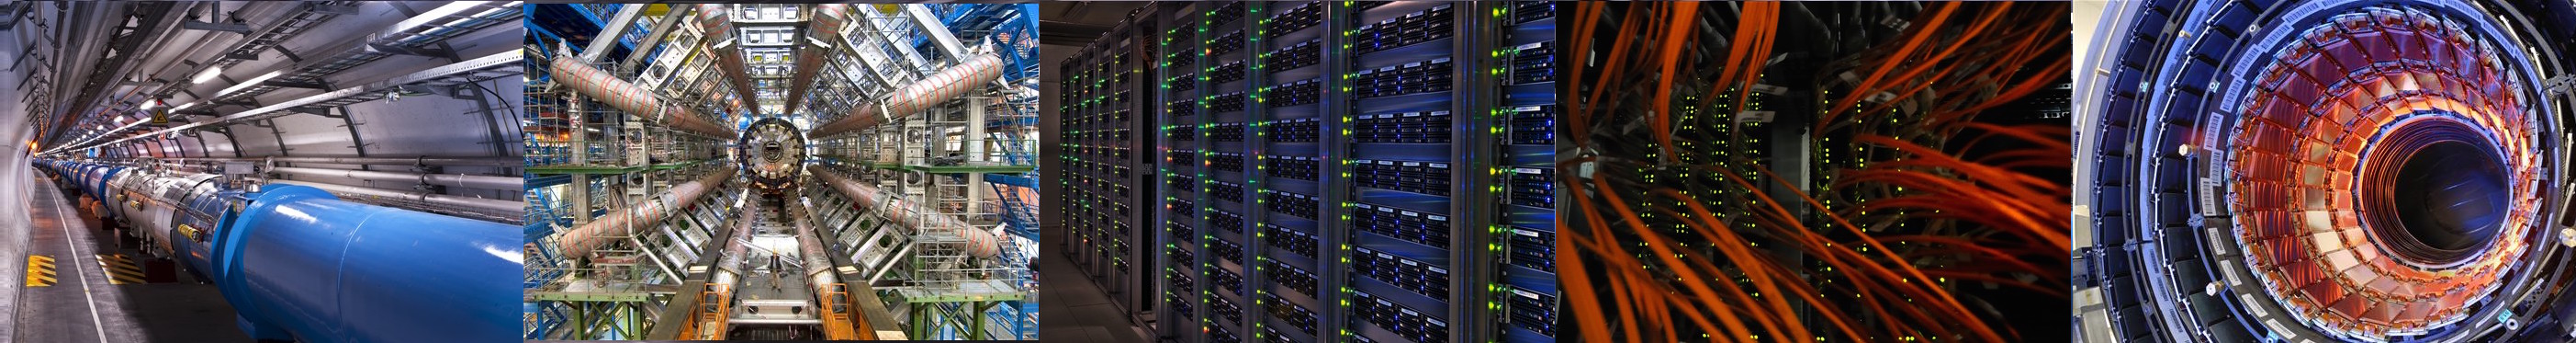
\includegraphics[width=1.0\textwidth]{images/s2i2-banner.jpg}
    \maketitle %this typesets the contents of \title, \author and \date
\vskip 4.1in
\begin{tabulary}{1.0\textwidth}{lr}

\includegraphics[width=0.1\textwidth]{images/nsf1.jpg} & \parbox{0.85\textwidth}{This document has been produced by the IRIS-HEP project (\url{http://iris-hep.org}) and supported by National Science Foundation grant OAC-1836650. Any opinions, findings, conclusions or recommendations expressed in this material are those of the project participants and do not necessarily reflect the views of the National Science Foundation.}
\end{tabulary}
}
\thispagestyle{empty}
\newpage

%\linenumbers
\thispagestyle{empty}
\tableofcontents
\newpage
\setcounter{page}{1}

%\input{002-revisions.tex}

\appendix
%\input{900-appendix-wbs-reporting.tex}

\newpage 
%\bibliographystyle{unsrt}
%\bibliography{irishep-pep}



\end{document}
